%Chapter 3: Rapid Static Modeling

%Vertical ellipsis in vectors is missing

\chapter{Rapid Static Modeling}

In the introductory chapter we discussed how recent response to large earthquakes is been hampered by a strict reliance on seismic data for early characterization of the seismic source. In Chapter 2 we discussed briefly the problems facing traditional seismological instrumentation at local and regional distances of large events. Seismometers clip during strong shaking and strong motion sensors are beleaguered by baseline offsets. The latter problem, baseline offsets, is particularly important because it affects the long period band of seismic time series. It's precisely this frequency band that is most useful for discerning the broad features of large earthquakes. If a geophysical instrument is band limited then it will become increasingly difficult to differentiate between say a magnitude 7 and a magnitude 8 event. This is a condition known as saturation and it's common in early warning algorithms that rely on seismometers and accelerometers alone\cite{Brown2011}.

Large events induce a permanent deformation of the Earth's crust, the static field. If the earthquake is large enough, and the geophysical sensor close enough or sensitive enough it's possible to measure the static field. For hazards applications this is of great interest because the static field is a zero frequency wave and as such the longest period information we can measure about an event. Thus characterization of the static field and of its contribution to a seismogram solves the problem of saturation. Furthermore the static field can be to first order assumed to have no time dependence, this makes it simple to extend earthquake source models from point sources to more realistic and complex geometries without consideration for the time-dependent effects of linear superposition.

Although noisier than accelerometers, GPS can easily record the permanent deformation at regional distances of large earthquakes, this was documented as far back as the 1992 M7.2 Landers earthquak \citep{bock1993,blewitt1993}.  It has since become routine to observe coseismic offsets in post-processed GPS time series after medium to large events and discussion in the literature of the potential of static filed modeling for rapid response has become vigorous. \citet{Blewitt2006} showed that given an epicentral location and assuming thrust faulting for the 2004 Mw 9.2  Sumatra-Andaman earthquake, one could have estimated an accurate magnitude within 15 minutes of the origin time using global GPS stations at regional to teleseismic distances. \citet{sobolev2007} proposed and demonstrated the viability of a system that uses coseismic offsets from GPS to directly invert for a heterogeneous slip model. \citet{Crowell2012} produced heterogeneous coseismic slip inversions from real-time data for two large events and \citet{Wright2012} produced source models with 4 fault patches from precise point positioning data for the M9 Tohoku-oki earthquake. \citet{Ohta2012} were able to produce in simulated real-time mode a simple uniform slip source model for the 2011 Tohoku-oki event and discussed the viability of using such a model to simulate tsunami propagation. \citet{PerezCampos2013} computed similar models for one scenario and one recorded subduction event in Mexico with a sparse network. This patchwork of studies demonstrate to varying degrees the viability, interest and importance of rapid modeling algorithms that employ the static field.

Throughout this chapter we will demonstrate a coherent framework that demonstrates how such recordings can be used. We will demonstrate the logical progression from point source CMT models to finite extent MT's and finally slip inversions.

The Kalman filter method discussed in the previous Chapter aides these algorithms insofar as it allows for better quantification of static offsets. Most notably there can be an order or more magnitude improvement in the resolution of vertical offsets. Nonetheless, its net effect, while non-negligible, is not of paramount importance. Many of the methods discussed in this Chapter can be quite successful with GPS data alone. Later on in Chapter 4 we will see the true benefit of the filtered data for source estimation when we compute kinematic models. However, when pertinent, we will demonstrate the improvements to the results as a consequence of the filtering operation.

\section{Centroid Moment Tensor Inversion}
\label{sec:cmt}

Computation of the seismic moment tensor (MT) for a given earthquake is one of the fundamental kinds of modeling performed to study the earthquake source. The moment tensor can be calculated from a number of methods such as polarity of first arrivals \citep{Havskov2010} or waveform matching \citep{dreger2003} and is a compact representation of the source that contains basic information on the size of the event, the fault plane geometry and the style of faulting. Moment tensor solutions are of use over a range of earthquake magnitudes. Small to medium events are utilized for tectonic studies and to determine the stress regime within a region. For large events, rapid determination of the centroid location as well as the moment tensor (CMT) provides valuable information for earthquake response, tsunami early warning and as a starting point for finite fault source modeling.

Currently there are a number of efforts that routinely compute moment tensor solutions for earthquakes worldwide. The most comprehensive catalogue of such solutions is contained in the Global Centroid Moment Tensor (GCMT) Project. At its inception the GCMT project included inversion of body and surface waves \citep{dziewonski1981,dziewonski1983} and has seen numerous refinements since such as inclusion of aspherical Earth structure, attenuation, etc. This method however employs only teleseismic data and its emphasis is in data collection and catalogue compilation not in rapid modeling. Real-time moment tensors can be obtained for small to medium events using time domain waveform matching inversion schemes  \citep{dreger1990,dreger1993}. However, real-time CMT determination of medium to large events is still an active area of research.

One of the most important advances in computing CMTs as quickly as possible for large events is contained in the work of \citet{kanamori2008} who elaborated on \citet{kanamori1993}'s observation of the W phase, a long period phase arriving in between the direct P and S waves. They showed that inversion for the moment tensor using data as close as 15 from the source is viable. W phase inversion algorithms currently run in real time at the USGS, Pacific Tsunami Warning Center (PTWC) and Institut du Physique du Globe de Strasbourg (IPGP-EOST) \citep{hayes2009}. Since the W phase arrives well before large amplitude surface waves and remains on-scale far longer such inversion algorithms have shown to be a marked improvement in rapid computation of moment tensor solutions for large events over traditional waveform matching techniques. 

Following the Mw 9.0 Tohoku-oki earthquake,\citet{duputel2011} showed that it was feasible to use data at distances as small as 11$^\circ$ from the source. However, W phase based inversion schemes, while very robust, require long period displacement records (e.g. 200-1000s for the 2011 Tohoku-oki event) \citep{duputel2011}. Such recordings, as discussed before, are almost always unusable close to the source in real time; velocity instruments clip and it is difficult to extract long period motions from strong-motion accelerometer data in real time.

Thus, there seems to be a limitation in how fast moment tensor solutions can be obtained operationally for large events using seismic instruments and existing seismological methods. For example, for the Tohoku-oki event it took 20 minutes after origin time to arrive at the first CMT solutions by agencies running W phase algorithms \citep{duputel2011}, even though the rupture had a duration of three minutes \citep{simons2011}. This delay was due to the reliance on teleseismic data. After several iterations using progressively more data, the final CMT solution \citep{hayes2011} was obtained 90 minutes after origin time using data up to 90 from the rupture. The first estimate of moment magnitude was obtained in about 3 minutes by the Japan Meteorological Agency (JMA), but was grossly underestimated at Mw=6.8. \citep{duputel2011} documented that in the numerous iterations between agencies the nodal planes were somewhat consistent with only minor variations in strike dip and rake, the magnitudes oscillated between Mw 8.8-9.0 after the 20-minute mark, but the centroid locations varied by as much as 2 and 60 km in depth.ing 

\subsection{Extracting Coseismic Offsets}

Our inversion schemes use coseismic offsets, we apply a 120 s moving average filter to the 1 Hz displacement waveforms to remove the dynamic component and retain the information on the permanent deformation. GPS data have much higher noise levels than traditional seismological data sets in particular in the vertical direction, thus, we set a threshold of 15 mm on the total horizontal component at a given station. This is roughly 3 times the usual noise level in the horizontal component of real-time GPS measurements \citep{genrich2006}.  At any given epoch only stations over this threshold are considered for the inversion.
%Moivng/trailing variance stuff here

\subsection{Point Source Models}

We present a robust method for determining CMT solutions that is considerably faster than current seismic methods, based on real-time high-rate displacement data from near-source GPS stations. Although we are not explicitly solving for the style and geometry of faulting, that information is implicit in the moment tensor solution. In general, we do not require prior knowledge of the sense or extent of faulting, although that information could be used if available.
We demonstrate the new algorithm by replaying the estimation of 1 Hz displacements for the 2003 Mw 8.3 Tokachi-oki earthquake using GPS data from Japan�s GPS network (GEONET) \citep{Miyazaki1998} and for the 2010 Mw 7.2 El Mayor-Cucapah earthquake using data from the California Real Time Network (CRTN) \citep{Bock2004}. We will also discuss the limitations of the point source strategy as  illustrated by the Mw 9.0 Tohoku-oki earthquake.

\subsubsection{Inversion Scheme}

The inversion scheme employed here relates the coseismic offset measured at the surface to source parameters at depth. \citet{Amoruso2004} and \citet{Hearn2005} showed that crustal layering can have a significant effect when inverting for source parameters using static offsets, thus we must account for, at least, a simple one-dimensional structure. To do so we compute Green�s functions (GFs) using Fortran codes EDGRN/EDCMP \citep{wang2003} for a 1D layered Earth. This numerical approach starts from the closed form solutions of the partial differential equations of motion obtained from the Hankel transform and then applies a Thomson-Haskell propagator matrix to relate the deformation at depth with that at the surface. We extract the GFs from the code output and set up the kernel matrix G for the inversion :
\begin{equation}
\left(\begin{matrix}
 u_1^1\\
 u_2^1\\
 u_3^1\\
 \cdot\\
 u_1^n\\
 u_2^n\\
 u_3^n\\
\end{matrix}\right)
=
\left(\begin{matrix}
G^1_{11} & G^1_{12} & G^1_{13} & G^1_{14} & G^1_{15}\\
G^1_{21} & G^1_{22} & G^1_{23} & G^1_{24} & G^1_{25}\\ 
G^1_{31} & G^1_{32} & G^1_{33} & G^1_{34} & G^1_{35}\\
\cdot &  &  &  & \cdot\\
G^2_{11} & G^2_{12} & G^2_{13} & G^2_{14} & G^2_{15}\\
G^2_{21} & G^2_{22} & G^2_{23} & G^2_{24} & G^2_{25}\\ 
G^2_{31} & G^2_{32} & G^2_{33} & G^2_{34} & G^2_{35}\\
\end{matrix}\right)
\left(\begin{matrix}
 m_1\\
 m_2\\
 m_3\\
 m_4\\
 m_5\\
\end{matrix}\right)\;,
\end{equation}
or more succinctly
\begin{equation}
\label{eq_mshort}
u_i^k=G^k_{ij}m_j\;;\;\{i=x,y,z\;,\;j=1,2,\dddot,5\;,\;k=1,2,\dddot,n\}\;,
\end{equation}
where $u_i^k$ is the $i$th component of displacement measured at the $k$th station, $m_j$ is the $j$th component of the moment tensor and $G_{ij}^k$ are the $i$th component GFs that relate the $j$th component of the moment tensor to the $k$th station. Thus the GF matrix is very compact, having only 5 elements per direction of motion per station.

The moment tensor in this case is composed of 5 components since we restrict the inversion to the deviatoric portion such that for the general six component symmetric Cartesian MT
\begin{equation}
\label{eq_mcart}
\mathbf{M}
=
\left(\begin{matrix}
m_{xx} & m_{xy} & m_{xz}\\
m_{xy} & m_{yy} & m_{yz}\\
m_{xz} & m_{yz} & m_{zz}\\
\end{matrix}\right)\;,
\end{equation}
the deviatoric restriction means that the following equivalences between equations Equations \ref{eq_mshort} and \ref{eq_mcart} hold
\begin{eqnarray}
m_1=m_{xy}\nonumber\\
m_2=m_{xz}\nonumber\\
m_3=m_{zz}\nonumber\\
m_4=(1/2)\dot(m_{xx}-m_{yy})\nonumber\\
m_5=m_{yz}\;.
\end{eqnarray}
We have retained the \citet{Aki2002} convention where $x$ is north, $y$ is east and $z$ is down. This is just one of many possible moment tensor coordinate representations; however we have chosen this one to be consistent with the notation used by the EDGRN/EDCMP software.

Since we are making a point source approximation and neglecting fault finiteness, we assume that despite the coseismic motions the source to receiver distances remain unchanged and so the Green�s function matrix remains unaltered throughout the inversion process. Next we assemble the data vector from that epoch�s measured coseismic offset and weigh the data by the pre-event standard deviations as
\begin{equation}
\textbf{Wu}=\textbf{WGm}\;,
\end{equation}
where
\begin{equation}
\textbf{W}=\mathrm{diag}\left(
\frac{1}{\sigma_1^1},\frac{1}{\sigma_2^1},\frac{1}{\sigma_3^1},\frac{1}{\sigma_1^2},\frac{1}{\sigma_2^2},\frac{1}{\sigma_3^2},\dddot  ,\frac{1}{\sigma_1^n},\frac{1}{\sigma_2^n},\frac{1}{\sigma_3^n}\right)\;,
\end{equation}
and the  $\sigma_i^k$�s are the standard deviations obtained from 60 s of pre-event noise at the $k$th station on the $i$th channel. This is a reasonable assumption since, in the absence of motion, the pre-event time series are many realizations of a zero measurement. The weight matrix remains constant across all epochs, since we assume that the noise characteristics of the GPS time series are the same for the duration of the inversion. The noise characteristics of real-time GPS displacements should be stable on the scale of minutes \citep{genrich2006}. Furthermore in Chapter 2 we saw no found no appreciable increase in the noise level between quiescent periods and periods of shaking during the shaketable tests. Thus, to first order, the noise can be assumed to be constant for the duration of strong shaking.

An additional weighting is applied based on the distance $r$ from the source to the receiver. Because the static field decays according to  $1/r^2$ \citep{Aki2002} we divide each time series by a weight $w_r$ to avoid having the largest offsets overwhelm the norm minimized by the inversion. This is a technique analogous to the one used in time domain waveform moment tensor inversion \citep{dreger2003}.  For a centroid to station distance $r_i$ the weight is defined as
\begin{equation}
w_r^i=\frac{[\mathrm{min}(r_i)]^2}{r_i^2}\;,
\end{equation}
thus, we have two weighting factors, one that determines how trustworthy an offset is when compared to background noise levels and a second one that ensures that the largest offsets do not dominate the inversion.

The inversion is performed at each time step (once per second in this case) utilizing the coseismic offset measured at that epoch to produce a new moment tensor. We experimented with L2-norm inversion using a QR decomposition and L1-norm inversion \citep{Boyd2004}. We found that L1-norm minimization converges to a stable solution before the L2-norm inversion.

For analysis of the inversion we obtain the seismic scalar moment $M_0$ as the scaled Frobenius norm of the moment tensor \citep{Silver1982}
\begin{equation}
\|\mathbf{M}\|=\frac{1}{\sqrt 2}\left(\sum_{i=1}^{3}\sum_{j=1}^{3}M_{ij}^2\right)^{1/2}\;,
\end{equation}

to then compute the moment magnitude using the relationship of \citet{Hanks1979}. Additionally we compute the deviation of the model from a pure double couple source as gauged by the parameter $\epsilon$ \citep{dziewonski1981} which is computed from the moment tensor eigenvalues as
\begin{equation}
\epsilon=\frac{\gamma_{min}}{\gamma_{max}}\;,
\end{equation}
where $\gamma_{min}$ is the smallest eigenvalue in the absolute sense and $\gamma_{max}$ is the largest. $\epsilon=0$ denotes a pure double couple source and $\epsilon=0.5$ a pure compensated linear vector dipole (CLVD) source.

The hypocenter and centroid locations can vary substantially since the hypocenter is the point of initiation of rupture while the centroid is the point of mean moment release. The hypocenter can be determined rapidly from traditional seismic data but the centroid location is harder to compute. To locate the centroid we employ a grid searching approach by defining a discrete grid around the stations that first detect the coseismic offsets. We invert simultaneously at each epoch on all grid points (inversion nodes) assuming that each node is the centroid. We then compute the misfit of the inversion at each node and define the final centroid location for that epoch as the one with the largest variance reduction (VR):
\begin{equation}
\mathrm{VR}=\left(1-\frac{\sum_{i=1}^n[d_i-(\mathbf{Gm})_i]^2}{\sum_{i=1}^n d_i^2}\right)\times100\;.
\end{equation}

In order to build the grid of nodes on which the inversion will take place, it's possible to use a precomputed slab model (in the case of subduction zone events) or have a library of fault surfaces (for strike slip environments) as a template for a grid. Alternatively it's possible discretize the known geological surfaces to define the inversion nodes thus forcing the centroid to lie on known faults. We prefer to minimize assumptions and simply build a sufficiently large three dimensional prism of grid points around a preliminary hypocentral location. The choice of strategy will depend on the observational goals of a network. In any case, we combine a formal inversion with a grid search to solve for the CMT using an algorithm that we call \textit{fast}CMT.

\subsection{Demonstration}

To demonstrate our approach, we apply here the \textit{fast}CMT algorithm for a subduction zone earthquake and for an earthquake in a strike-slip environment, using near-field 1 Hz GPS network data replayed in a simulated real-time mode to estimate displacements. 

\subsubsection{2003 Mw 8.3 Tokachi-oki Earthquake}

The first example of \textit{fast}CMT is for the 2003 Mw 8.3 Tokachi-oki earthquake. This megathrust event ruptured a segment of the Kuril-Japan trench, sharing most of the source area and rupture characteristics of the 1953 Mw 8.1 Tokachi-oki earthquake \citep{Hamada2004}. We estimated displacements in simulated real-time mode for 300 seconds of GEONET 1 Hz data from 355 stations in Honshu and Hokkaido islands. Some very near source stations lost telemetry and have incomplete records so we excluded those from processing. We applied a 120 s moving average to each displacement record in each coordinate component to extract the permanent deformation from the displacement waveforms; the resulting time series can be seen in Figure \ref{fig_toki_tseries}. The static offset at the stations closest to the source is discernible at around 160 s. As is usual with GPS time series, the vertical component is noisier than the horizontals \citep{genrich2006}.

\begin{figure}[!ht] 
  \centering
  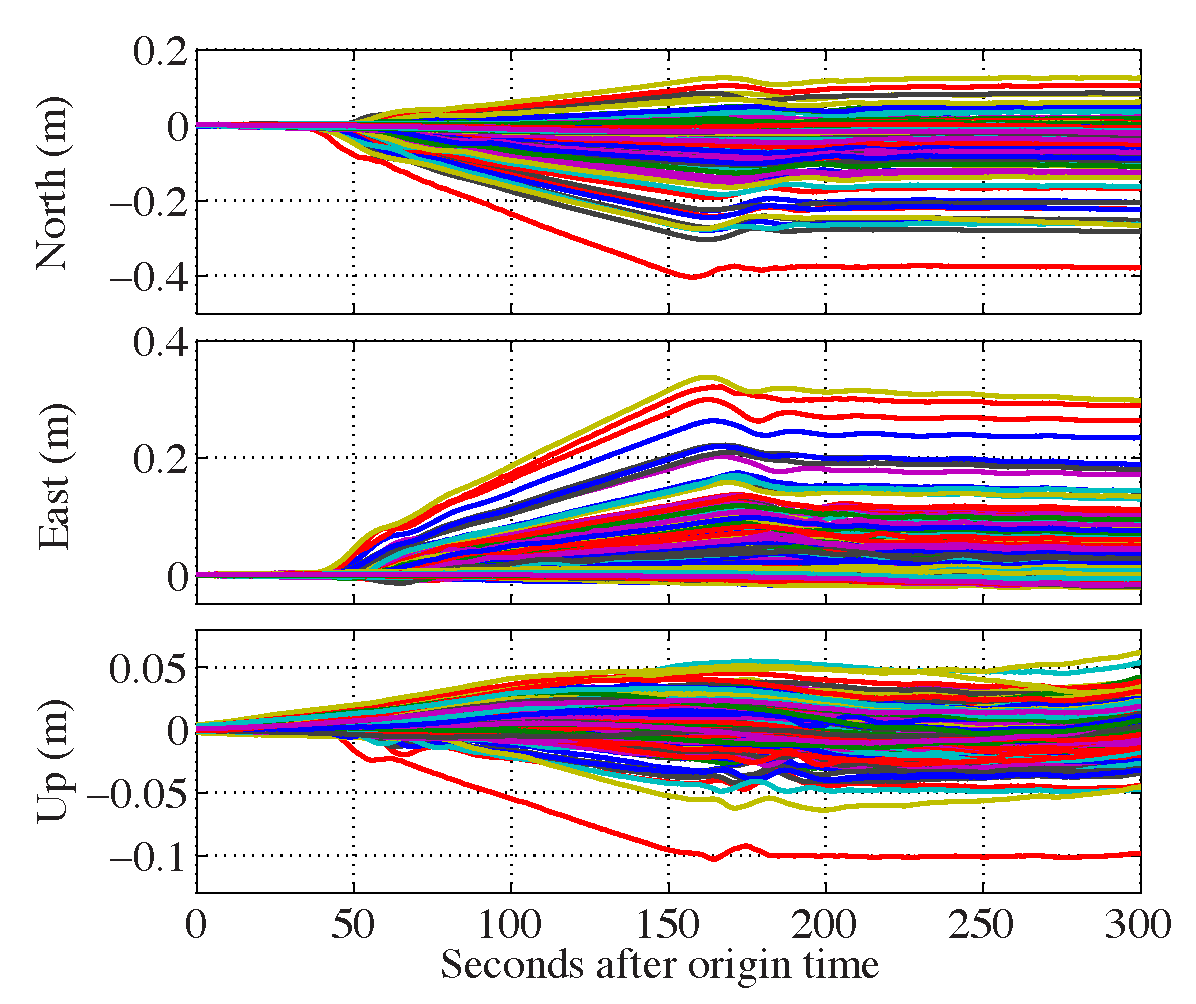
\includegraphics[width=0.88\linewidth]{./figures/ch3/toki_tseries.pdf}
    \caption[Tokachi-oki GPS time series]{First 300 s of displacement records at 355 GEONET stations with a 120 s moving average filter applied for the Tokachi-oki earthquake.}
  \label{fig_toki_tseries}
\end{figure}

Green�s functions were computed from EDGRN on a 1 km horizontal and vertical grid using the four-layer velocity model employed by \citet{Yagi2004} for near source slip inversion (Table \ref{tb_toki_model}). This is a much denser coverage than the actual station distribution, thus, at any given station the resulting GF is the spline interpolation of the closest grid points. For this scenario we used a 3-D 3$^\circ\times$3$^\circ$ prism of gridpoints spaced at 0.2$^\circ$ and every 3 km in depth between 3 and 60 km centred around the mean latitude and longitude of the first stations to meet a detection criterion.

\begin{table}
\caption{Velocity model for the Tokachi-oki inversion}
\label{tb_toki_model}
\begin{tabular}{l r r r r}
\hline
Layer & $v_p$ & $v_s$ &Density&Thickness\\
 & (km/s) &( km/s) & (kg/m$^{3}$) & (km)\\
\hline
1 & 3.80 & 2.19 & 2.30 & 4.0\\
2 & 5.50 & 3.18 & 2.60 & 4.0\\
3 & 5.80 & 3.34 & 2.70 & 10.0\\
4 & 6.50 & 3.74 & 2.90 & 10.0\\
Half-space & 7.80 & 4.50 & 3.20 & $\infty$\\
\hline
\end{tabular}
\end{table}

% 
defined the criterion that displacements from 5 stations over the 15 mm threshold are required to start the inversion; for the 2003 Tokachi-oki event this occurred at 43 s after origin time. The results of the inversion are shown in Figures \ref{fig_toki_centroid_loc} and 3. Figure 2 shows the centroid determination as a function of time as well as the estimated magnitude and the parameter ?; Figure 3 shows snapshots of the resulting CMT (the full result is in supplementary movie S1) as well as the observed and synthetic horizontal displacements. Figure 2 shows that by 50 s a rough centroid location is available with oscillations between adjacent nodes. The magnitude reaches Mw 8.0 at 75 s, with a 75\% variance reduction. However, as evidenced by the time series (Figure 1) the full coseismic offset has not yet occurred. The magnitude continues to grow and settles at 8.3 by 170 s. The plot of the variance reduction also shows that at 200 s (when the final offset is in place) the fit to the data is maximum (85\%) degrading towards the end of the inversion. Figure 3 and supplementary movie S1 show the oscillation between adjacent nodes for the centroid solution and also indicate how by 65 s a thrusting mechanism is already resolved although the magnitude is still underestimated. However, by 180 s and onwards the inverted mechanism is close to that of the GCMT solution (http://www.globalcmt.org/). Variance reduction values are computed at every epoch (supplementary movie S2 shows the evolution of this misfit function for the full 300 s). To illustrate the grid searching method, Figure 4 shows a snapshot of variance reduction at 180 s after the origin time.

\begin{figure}[!ht] 
  \centering
  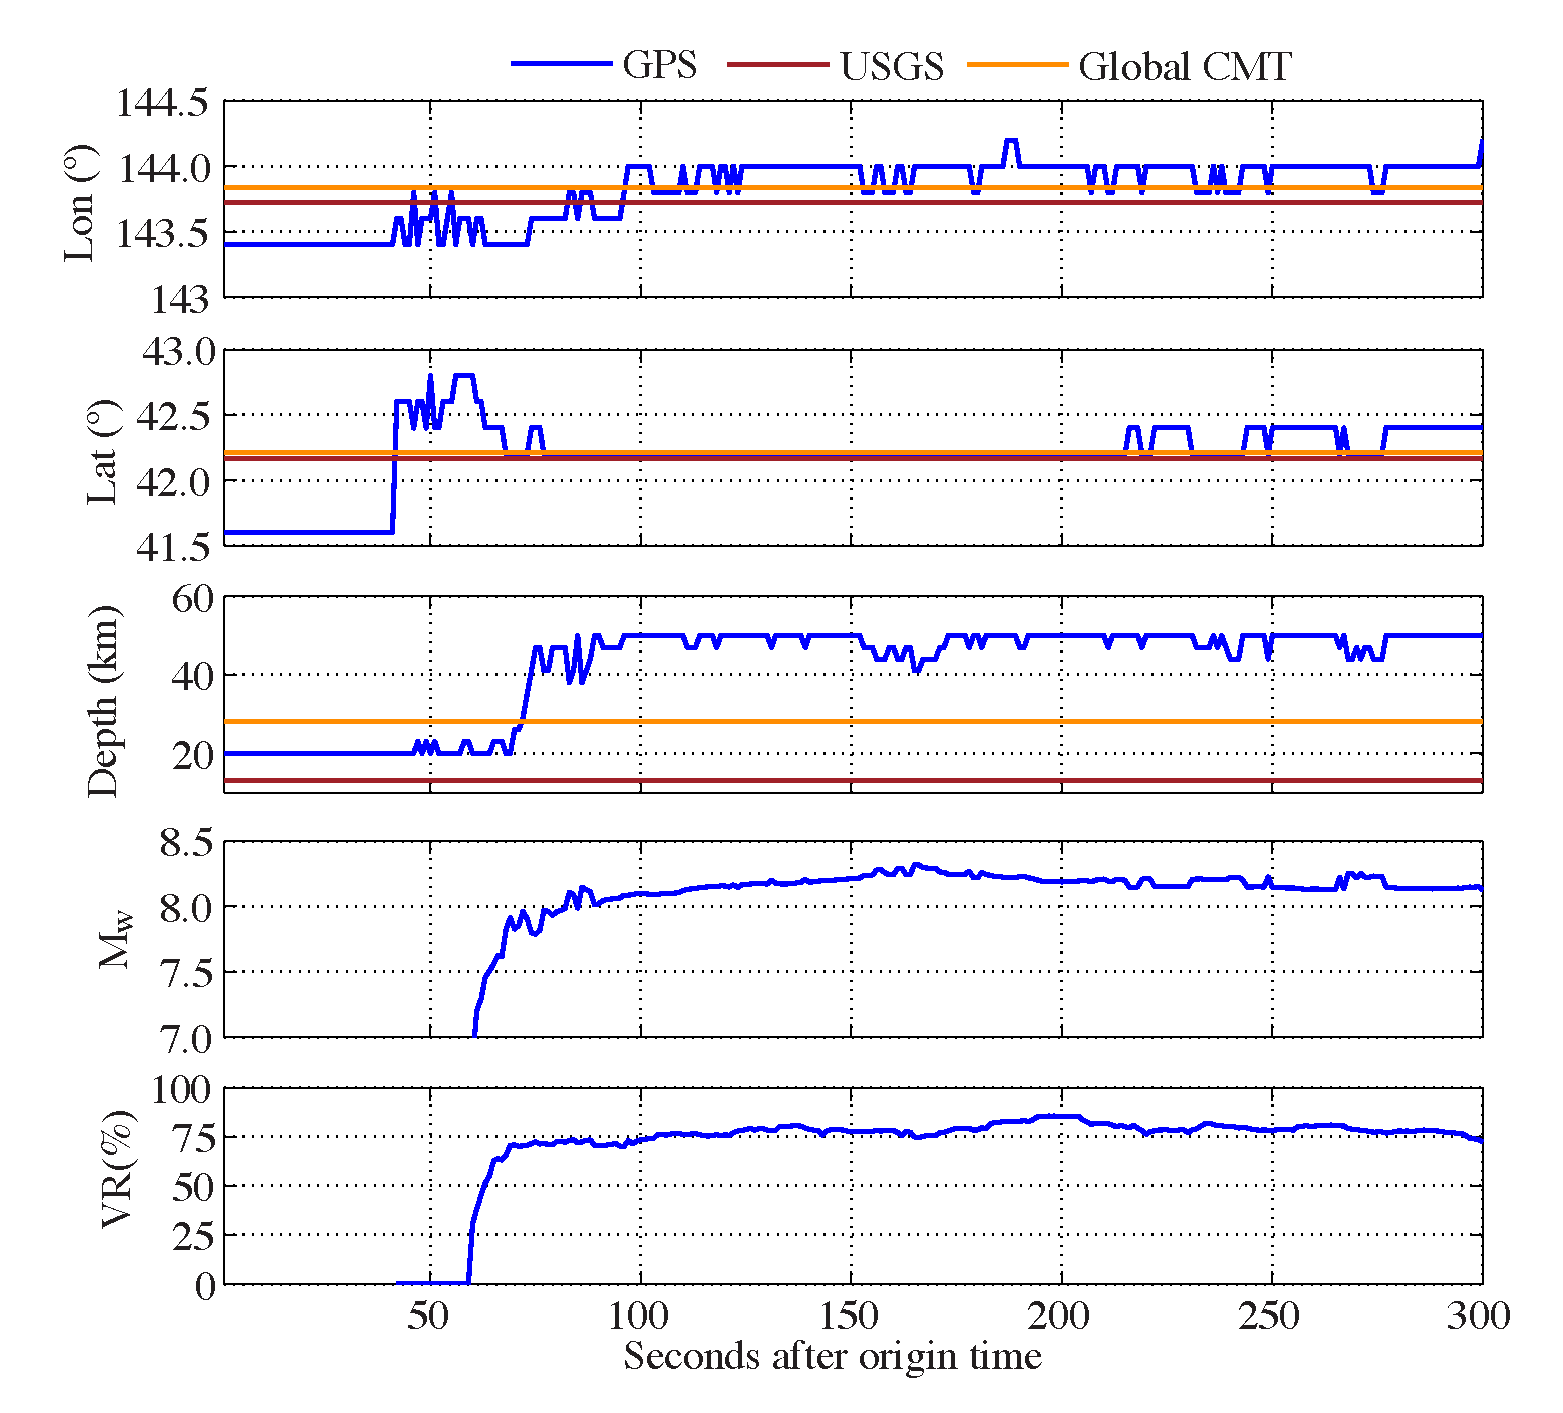
\includegraphics[width=0.88\linewidth]{./figures/ch3/toki_centroid_loc.pdf}
    \caption[Tokachi-oki inversion summary]{Summary of the inversion results for the Tokachi-oki earthquake. The top three panels are the centroid determination as a function of time compared to the location reported by the USGS and the Global Centroid Moment Tensor Project. The fourth panel is the computed magnitude and the fifth panel is the misfit (variance reduction)}
  \label{fig_toki_centroid_loc}
\end{figure}

	To further evaluate the quality of the solution we extracted the strike, dip and rake of the nodal planes from the moment tensor solution every second by decomposing it into its best double couple. The results are shown in Figure 5 and compared to the GCMT results. They illustrate that the geometrical parameters of the best double couple are well determined at 65 s  before the end of rupture and full coseismic deformation occurs and remain fairly similar to the post-processed  GCMT solution throughout. Furthermore the size of the CLVD is fairly small throughout the inversion, never exceeding     ? = 0.05.


 


%\appendix
%\chapter{Final notes}
%  Remove me in case of abdominal pain.

